\section{The Algorithm}
\subsection{Knowledge Distillation}
All the paper work is based on knowledge distillation, which is a technique that allows a neural network to distil knowledge from a master neural network, without knowing anything about the dataset.\\ 
This process has been studied previously in some papers\cite{kd}\cite{fokd}\cite{tkd}, but with the sole purpose of building a lighter and simpler student model that could be used in a production environment, starting from a much more complex master, but also keeping good performances.\\
In the reference paper the idea is to use the same technique but this time applying it to the same model or to a model of comparable complexity. What we saw is that often the student model was superior to the master. All this seems to be the result of a more complete information contained in the output of the master model, in fact it does not only provide a negative or positive value for each class of reference, but also a probability distribution that makes the model aware of how two classes are "close" and "confusable".\\
There are different ways to work with knowledge distillation, that is why I decided to have an implementation as generic as possible. So I coded a method that would take in input a dataset, a teacher and a student. As a first step the dataset is encapsulated in a custom generator that iterating returns the as $X$, the same as the dataset, and as $y$, instead of ground truth, the prediction of the master.\\
But now let's see the code:
\lstset{language=Python}
\lstset{frame=lines}
\lstset{caption={The code for distilling knowledge}}
\lstset{label={lst:code_direct}}
\lstset{basicstyle=\footnotesize}
\begin{lstlisting}
def distil_knowledge(teacher_model, student_model, train_dataset, 
                      fit_args, ground_truth_weight=None):
  if (ground_truth_weight is not None and (ground_truth_weight > 1 or ground_truth_weight < 0)):
    raise ValueError("Please check the ground truth weight")
  def custom_generator(train_dataset, t_model, ground_truth_weight):
    for (x, y) in train_dataset:
      y_targets = teacher_model(x)
      if ground_truth_weight is not None:
        y_targets = (1-ground_truth_weight)*y_targets+(ground_truth_weight)*y
      yield (x, y_targets)

  s_history = student_model.fit(custom_generator(train_dataset, 
                                                 t_model=teacher_model,
                                                 ground_truth_weight=ground_truth_weight),             
                                                 **fit_args)

  return s_history
\end{lstlisting}

The idea is simple, the training happens like any other model, but the labels are passed by a generator, which will use the training dataset to get the teacher's predictions. In case you want to "weigh" the probability distribution with the ground truth, it will be enough to set the parameter "\textit{ground\_truth\_weight}".
\newpage
\subsection{Born Again Network}

The main algorithm presented in the paper\cite{ban} trains the teacher until convergence, after which, it initializes a student and uses the output of the master's softmax as the student's target. The process is repeated for several times, and it is observed that at some point there will be no improvement.\\
The study also indicates the possibility of improving performaces using an ensemble formed by the various generations of students. The output will therefore be an average of the students' output.

\begin{figure}[h!]
\centering
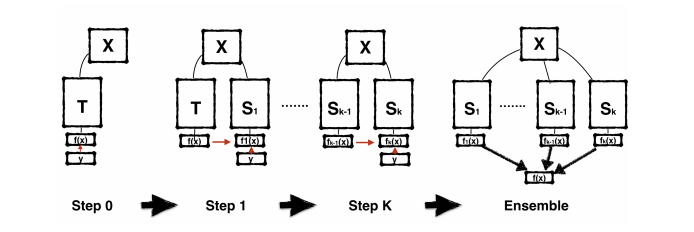
\includegraphics[width=1\textwidth]{ban.png}
\caption{Illustration of the algorithm, taken from the paper \cite{ban}}
\end{figure}
The implementation as the previous method, has to be as generic as possible, so, to achieve the result, we will have in input:
\begin{itemize}
\item The master model
\item The function to build the students in cascade
\item The parameters to compile the models.
\end{itemize}
In this way there will be the maximum freedom on the choice of the student.
\newpage
\lstset{language=Python}
\lstset{frame=lines}
\lstset{caption={The code for training a list of students}}
\lstset{label={lst:code_direct}}
\lstset{basicstyle=\footnotesize}
\begin{lstlisting}

def ban(teacher_model, n_students, build_model, 
        train_dataset, fit_args,
        checkpoints=False,
        ground_truth_weight=None,
        compile_args={'optimizer':'adam', 
                      'loss': 'categorical_crossentropy', 
                      'metrics': ['accuracy']}):
  students = [build_model() for i in range(n_students)]
  students.insert(0, teacher_model)
  for student in students:
    student.compile(**compile_args)
  history = []


  for i in range(1, len(students)):
    print("Training BAN-{}".format(i))
    current_callbacks = fit_args['callbacks']
    if checkpoints:
      current_callbacks.append(tf.keras.callbacks.ModelCheckpoint(f"student.{i}.h5"))
      fit_args['callbacks'] = current_callbacks
    current_history = distil_knowledge(students[i-1], 
                                        students[i], train_dataset,
                                        fit_args,
                                        ground_truth_weight=ground_truth_weight)   
    history.append(current_history)
  return history, students

\end{lstlisting}
The algorithm builds the students using the function that is passed, then compiles all the students in a list. Before starting the training, put the teacher model at the top of the list. The training basically starts from the second element using knowledge distillation with the previous element. The method will return the histories and an array of students.
\subsection{Knowledge Distillation integrations}
In one of the papers cited we can find an example of a different way to see knowledge distillation\cite{kd} Caruana and his collaborators have noticed that in some cases the lowest probabilities are so close to zero that they have almost no influence on the final result\cite{conf}. The strategy found is therefore to train the student on the logits of the master trying to minimizing the "mean squared error".\\
Another way to deal with the problem is to use a temperature variable in order to get a softened result, on which you can then effectively minimize crossentropy. So the soft-max with temperature $T$ will be calculated in this way:

\begin{equation}
q_i = \frac{\exp(z_i/T)}{\sum_j(\exp(z_i/T)}
\end{equation}

The paper\cite{kd} also introduces the possibility to use the ground truth to have a weighted average and get better results, also indicates that from empirical tests, assigning a lower weight to the ground truth produces better results.
\subsection{Ensemble}
Another technique mentioned in the paper\cite{ban} and which I think is worth replicating is the creation of an ensemble, obtained by the various generations of students. According to the researchers in several cases this technique allows for improvements in performance.\\
Let's see the code of the Ensemble:
\lstset{language=Python}
\lstset{frame=lines}
\lstset{caption={The code for the BAN-Ensemble}}
\lstset{label={lst:code_direct}}
\lstset{basicstyle=\footnotesize}
\begin{lstlisting}

class BANEnsemble(tf.keras.models.Model):
  def __init__(self, students, **kwargs):
    super(BANEnsemble, self).__init__(**kwargs)
    self.students = students
    self.len = len(students)
  
  def call(self, inputs):
    s_out = []
    for student in self.students:
      s_out.append(student(inputs))
      
    
    x = tf.keras.layers.Add()(s_out)
    x = layers.Lambda(lambda y: y/self.len)(x)
    return x

\end{lstlisting}

